\begin{recipe}
[ %
	preparationtime = {\SI{35}{\minute}},
%	bakingtime={\SI{1}{\hour}},
%	bakingtemperature={\protect\bakingtemperature{topbottomheat=\SI{280}{\celsius}}},
	portion = {\portion{2}},
	source = {chrusher}
    ]{Beans and Rice}

    \begin{figure}[p]
    	\centering
    	\makebox[\textwidth][c]{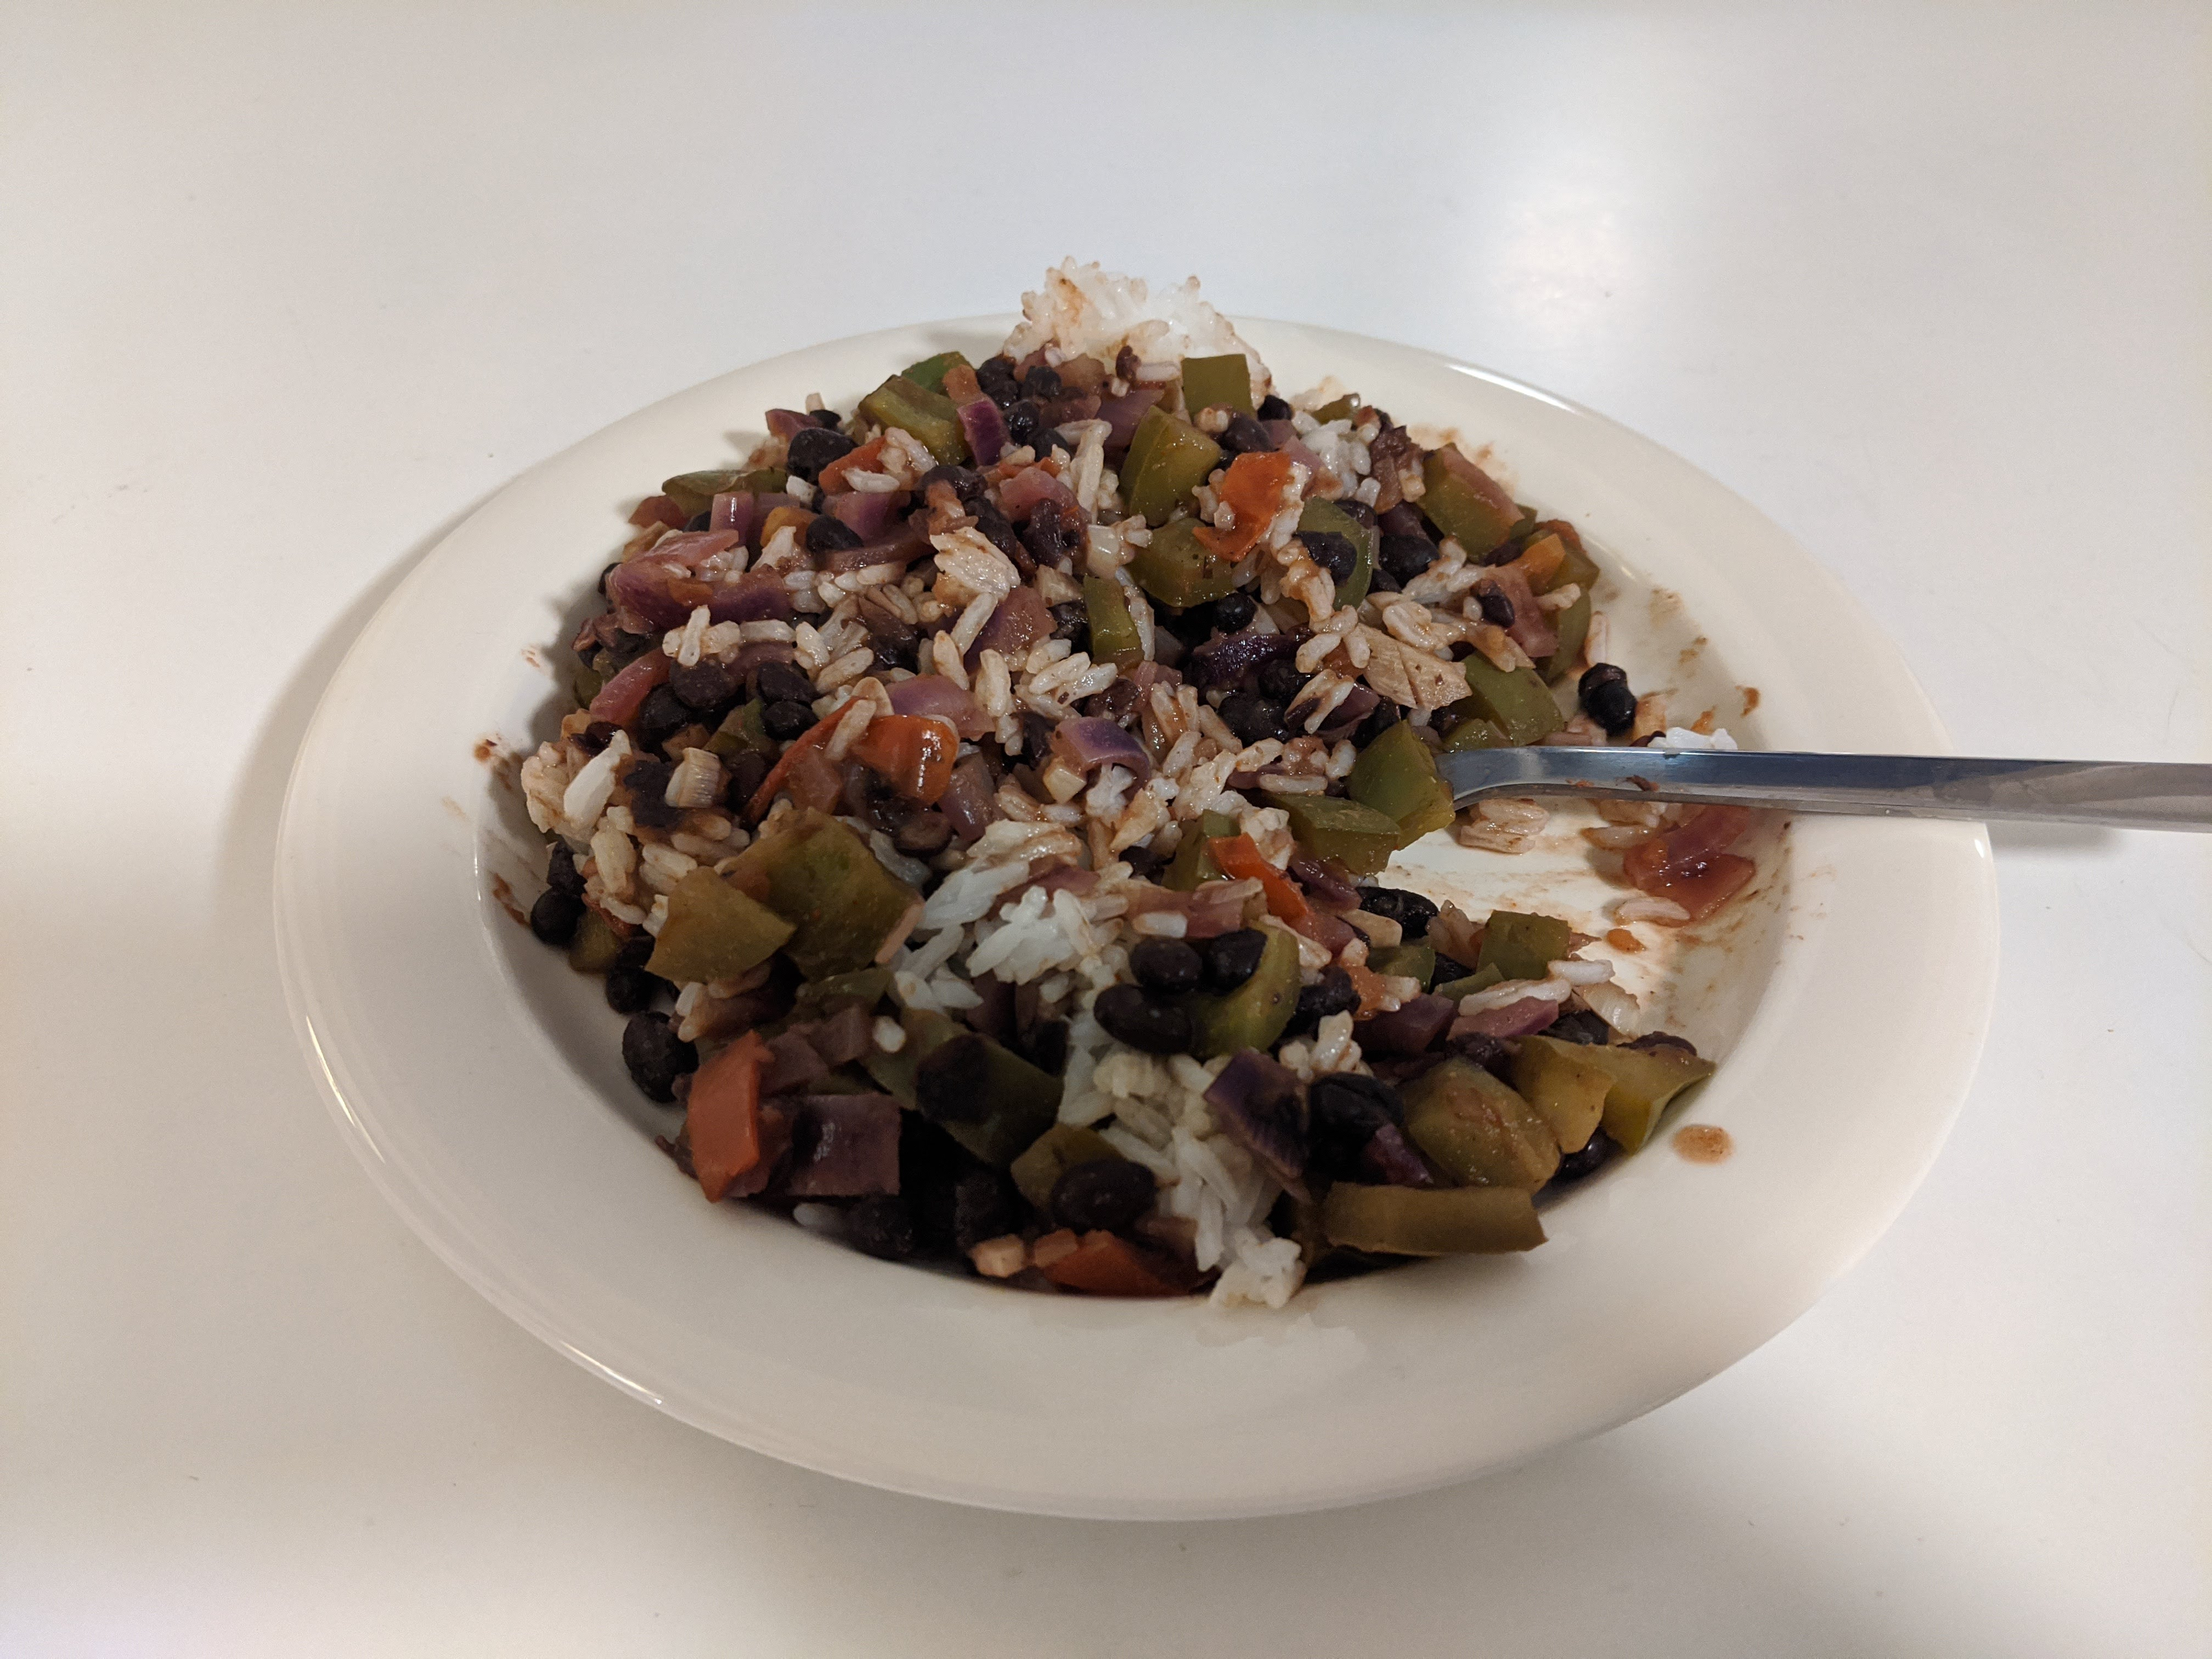
\includegraphics[height=\textheight]{beans_and_rice/IMG_20200422_211731.jpg}}
    \end{figure}

%    \introduction{
%
%	}

	\ingredients[15]{
		\SI{1}{can} & Black beans \\
		1 & Green pepper \\
		\SI{1}{small} & Red onion \\
		1 & Tomato \\
		& A few cloves of garlic \\
		\SI{125}{\milli\liter} & Rice \\
		\SI{500}{\milli\liter} & Water \\
		\SI{5}{\milli\liter} & Balsamic vinegar \\
		\SI{1}{\milli\liter} & Salt \\
		\SI{5}{\milli\liter} & Cajun seasoning or similar spice mix (it should have some cayenne or other chillies in it to provide some hotness)
	}

	\preparation{
		\step Cook rice your preferred method (I cook mine on the stove with one part rice to two parts water plus a dash of salt).

		\step Dice onion and green pepper before adding them to an oiled frying pan on medium heat.

		\step Peel and finely dice the garlic before adding them to the frying pan a few minutes after the pepper and onion.

		\step Drain and rinse the black beans before adding them to the pan a few minutes after the garlic.

		\step After a minute or two, add \SI{250}{\milli\liter} water then the vinegar and seasoning as well as the tomato, diced.

		\step Let the mixture cook on medium heat until most but not all of the water has boiled away.

		\step Serve the bean-vegetable mix on top of the rice.

		\vspace{1em}

		Vary the amounts of garlic, seasoning and vinegar to taste.
	}

\end{recipe}